\subsection{Indicadores Financieros}

Los indicadores financieros se basan en la comparación entre dos componentes esenciales de la información interna de una empresa: el balance general y el presupuesto. Mediante estos indicadores y su análisis, la organización puede definir el rumbo a seguir a partir de la evaluación de datos históricos.

Para este estudio se tuvieron en cuenta los siguientes indicadores financieros:

\begin{itemize}
    \item \textbf{Razón corriente: } Analiza la capacidad de la empresa para afrontar sus obligaciones utilizando los activos disponibles.
    
    \item \textbf{Nivel de endeudamiento total: } Mide el grado de participación de los acreedores en la estructura financiera de la empresa.
    
    \item \textbf{Rentabilidad operacional: } Indica el porcentaje de ingresos que se transforma en utilidades tras cubrir los costos operativos.
    
    \item \textbf{Rentabilidad neta: } Refleja la proporción de utilidades obtenidas respecto a las ventas netas, una vez descontados los costos fijos y variables.
    
    \item \textbf{Rentabilidad del patrimonio: } Mide las ganancias generadas a partir de la inversión de los accionistas.
    
    \item \textbf{Rentabilidad del activo:} Evalúa la rentabilidad de los activos de la empresa y su capacidad para generar beneficios a lo largo del tiempo.
\end{itemize}

La tabla \ref{indicadores} muestra la proyección de estos indicadores para los próximos 5 años.

\vspace{2mm}
\begin{minipage}{0.9\textwidth}
\centering
\captionof{table}[{Indicadores financieros}]{ Indicadores financieros}
\label{indicadores}
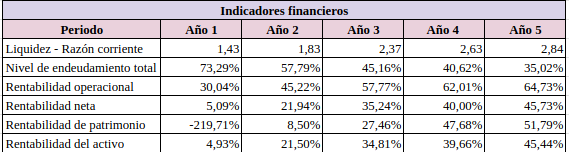
\includegraphics[width=0.9\textwidth]{Content/Images/AF/IndicadoresFinancieros.png}
\footnote{Nota. \textup{Fuente : Autores}}
\end{minipage}

Adicionalmente, se utilizaron los indicadores VAN, TIR y la relación costo-beneficio para evidenciar la factibilidad de la inversión desde la perspectiva de los accionistas. Los resultados se obtuvieron a partir del flujo de caja, cuyos datos se presentan en la tabla \ref{flujoLibre}.

\vspace{2mm}
\begin{minipage}{0.9\textwidth}
\centering
\captionof{table}[{Flujo de caja libre}]{ Flujo de caja libre}
\label{flujoLibre}
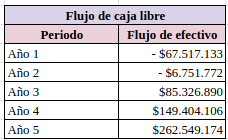
\includegraphics[width=0.9\textwidth]{Content/Images/AF/FlujoDeCajaLibre.png}
\footnote{Nota. \textup{Fuente : Autores}}
\end{minipage}

Considerando la tasa interna de oportunidad, que corresponde al rendimiento mínimo esperado por los accionistas, se estableció de manera subjetiva un valor del 10\% como compensación por la inversión.

En la tabla \ref{vanTIR} se resumen los resultados, evidenciando que la inversión se recupera en 5 años, superando los \$262.549.174 y multiplicando el capital inicial por más de cinco veces, con una tasa interna de retorno del 107\%.

\vspace{2mm}
\begin{minipage}{0.9\textwidth}
\centering
\captionof{table}[{VAN, TIR y RBC}]{ VAN, TIR y RBC}
\label{vanTIR}
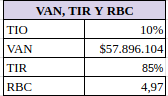
\includegraphics[width=0.9\textwidth]{Content/Images/AF/VanTirRbc.png}
\footnote{Nota. \textup{Fuente : Autores}}
\end{minipage}

El análisis de los resultados financieros respalda la viabilidad del proyecto. El éxito dependerá del interés de los inversionistas, lo que permitirá a la empresa expandirse en un mercado competitivo y con alta demanda. Tanto el Valor Actual Neto (VAN) como la Tasa Interna de Retorno (TIR) son positivos, y junto con una proyección de mayor liquidez según la tabla de ventas, se prevé una mejora significativa en la capacidad financiera de la empresa. Asimismo, se espera una disminución del endeudamiento y un crecimiento notable de la rentabilidad en los próximos años.
